% (C) 2013 - Université de Strasbourg
% * Guillaume Dollé <guillaume.dolle@math.unistra.fr>
% * Christophe Prud'homme <christophe.prudhomme@feelpp.org>
% Tutorial documentation - mymesh
%


\section{Mesh Manipulation}
\label{sec:mymesh}

Feel++ provides some tools to manipulate mesh. 
Here is a basic example that shows
you how to generate a mesh for a square geometry
(source \textcolor{magenta}{"doc/manual/tutorial/mymesh.cpp"}).
%
\vspace{2mm}
\lstinputlisting[linerange=marker_main-endmarker_main]{tutorial/mymesh.cpp}
\vspace{2mm}

As always, we initialise the \feel environment (see section \ref{sec:myapp}).
The \lstinline!unitSquare()! will generate a mesh for a square geometry.
\feel provides several functions to automate the GMSH mesh generation
for different topologies.
%
( \lstinline!unitCircle()!,
  \lstinline!unitCube()!,
  \dots ).
%
These functions will create a geometry file
\textit{.geo} and a mesh file \textit{.msh}. We can visualize them in GMSH. 
%
\begin{unixcom}
    gmsh <entity_name>.msh
\end{unixcom}
%
Finally we use the \lstinline!exporter()! function to export the mesh for post processing.
It will create by default a \textbf{Paraview} format file \textit{.sos} and an \textbf{Ensight}
format file \textit{.case}.
%
\begin{unixcom}
    paraview <app_name>.sos
\end{unixcom}
%
For advanced usage, there is the more generic \lstinline!createGMSHMesh()! function which is
useful for creating a mesh from a geometry. For loading a mesh, there is the loadGMSHMesh() function
(see section \ref{howto:spec-meshes} for a load example).
Note that \lstinline!unitSquare()! is just a particular case of \lstinline!createGMSHMesh()!.
\feel provide useful tools to iterate on the mesh or some faces that we will see later.
%
The process of the mesh creation is fully parallelized. You can as explained in section \ref{sec:myapp}
run this example on several processors and visualise subregions with paraview (see figures 
\ref{fig:tuto_mesh-1} and \ref{fig:tuto_mesh-2}).

\begin{figure}[!ht]
\centering
\subfigure{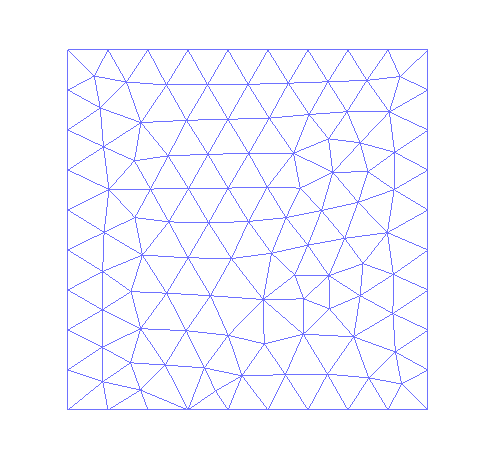
\includegraphics[width=4.5cm]{pngs/mymesh/hypercube_2.png}}
\subfigure{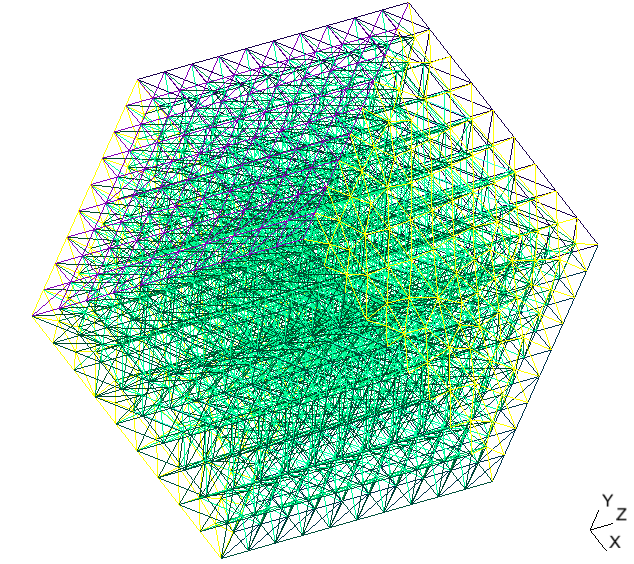
\includegraphics[width=4.5cm]{pngs/mymesh/hypercube_3.png}}
\caption{Mesh computed for square and cube geometries using one processor}
\end{figure}
\label{fig:tuto_mesh-1}

\begin{figure}[!ht]
\centering
\subfigure[Square and subregions]
    {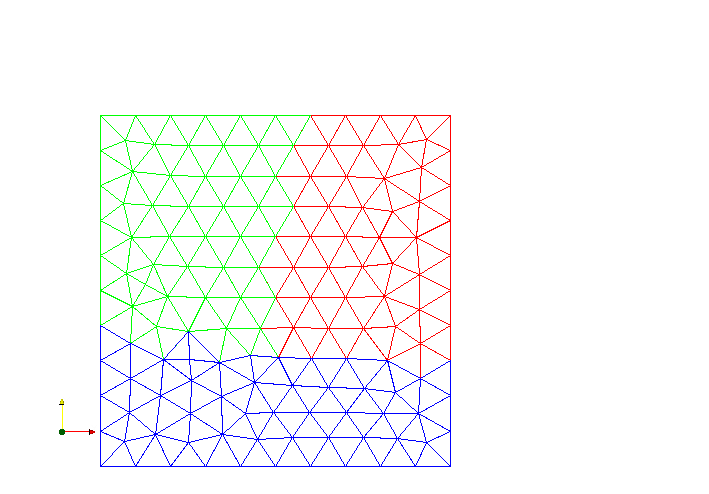
\includegraphics[width=6cm]{pngs/mymesh/mesh3.png}}
\subfigure[Cube and subregions]
    {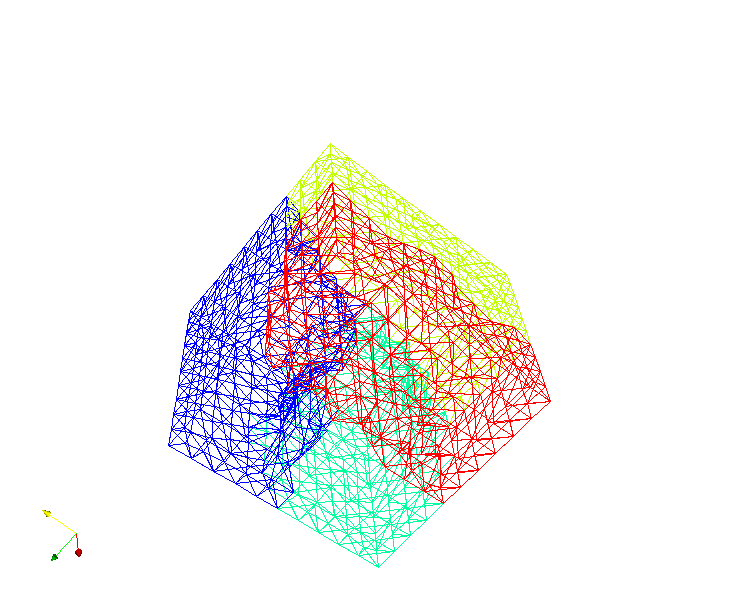
\includegraphics[width=6cm]{pngs/mymesh/mesh_cube.png}}
\caption{Mesh created for square and cube geometries using 4 processors}
\end{figure}
\label{fig:tuto_mesh-2}

%\begin{tikzpicture}
%\begin{axis}
%\addplot table[x=value1,y=value2]{tuto-mymesh-square.csv.save};
%\end{axis} 
%\end{tikzpicture}

